\section{Detección de la pelota}\label{chapter:deteccion}

La recopilación de información del medio ambiente, para detectar la posición de la pelota, se realiz\'o por medio de la cámara Raspberry Pi con el sistema operativo Raspian \cite{raspian}. Esta mini computadora y cámara constituyen una herramienta poderosa ya que permite capturar v\'ideos y fotos de alta definici\'on. Y como la Raspberry Pi cuenta con un procesador gr\'afico, este se encarga de manejar los datos de la cámara, aliviando la carga del procesador central \cite{raspCamArti}.

Además se ha decidido utilizar OpenCv \cite{opencv}, otra herramienta para procesar im\'agenes que se describe en la sección \ref{herramientasDetc}. Sin embargo los métodos de captura de OpenCV no funcionan con la c\'amara Raspberry Pi. En la secci\'on \ref{extraerImagen} se explica c\'omo se ha extra\'ido la imagen y en la secci\'on \ref{procesarImagen} se explica la forma en la que se ha procesado la imagen para hallar la posición de la pelota. 

\subsection{Herramientas software para la detecci\'on }\label{herramientasDetc}

Para extraer y procesar la imagen se utilizaron algunas librerias como apoyo. A continuación se presenta la descripción de la librería raspicam\_cv, usada para la extracción de la imagen y la descripción de la librería OpenCV, usada para la detección de la ubicación de la pelota.   

En visi\'on de computadoras existen varias liberias que apoyan y facilitan en procesamiento de im\'agenes, con herramientas de filtrado, transformaciones de im\'agenes, aprendizaje de m\'aquinas entre muchas m\'as. Dos ejemplos de ello son Processing \cite{processing} y OpenCv. Processing es un lenguaje de programaci\'on que está enfocado para iniciar a personas no programadoras en el \'area, por lo tanto explota la retroalimentaci\'on visual para atraer al usuario, posee herramientas de filtrado, de transformaci\'on de im\'agenes y muchas otras.
Por otro lado OpenCv (Open Source Computer Vision Library) es una librería de visión de computadoras y aprendizaje de máquinas de código abierto. Ha sido diseñada para acelerar el uso de la percepción de m\'aquinas y para proveer una estructura común en las aplicaciones de visión de computadoras \cite{opencv}. La decisi\'on de utilizar OpenCv se basa en su mayor amplitud de herramientas ofrecidas, un filtrado de im\'agenes mas amplio, un mayor control en el manejo de las im\'agenes y sus transformaciones.

Raspicam\_cv es una librería que permite obtener im\'agenes de la cámara Raspberry Pi en una estructura de datos compatible con OpenCV \cite{emilV}.

\subsection{Obtenci\'on de la imagen}\label{extraerImagen}

%<<<<<<< HEAD
%Dentro de las librerías oficiales para la cámara Raspberry Pi s\'olo se encuentran implemetadas en el lenguaje interpretado python y algunas aplicaciones para la línea de comandos de linux. Para utilizar la cámara con OpenCV en el lenguaje compilado \gls{C++} se requirió realizar una búsqueda de librerias alternas a las oficiales. Una primera solución se encontró en el blog de \cite{pierreR}, en donde explica que los métodos de captura de video de OpenCV no funcionan de manera nativa con el m\'odulo de la cámara de la Raspberry Pi (por ejemplo el método cvCapture). Para lograr extraer la imagen se basó en el código abierto de las aplicaciones raspivid y raspistill. Ha modificado el código para usar el buffer de la cámara y así obtener un objeto compatible con OpenCV. 
%raspicam\_cv es la librer\'ia utilizada en el proyecto que del c\'odigo ha sido moficicada convirtiendola una librer\'a por \cite{emilV}.
%=======
Dentro de las librerías oficiales para la cámara Raspberry Pi s\'olo se encuentran aquellas implemetadas en el lenguaje interpretado python y algunas aplicaciones para la línea de comandos de linux. Los métodos de captura de video de OpenCV no funcionan de manera nativa con el m\'odulo de la cámara de la Raspberry Pi (por ejemplo el método cvCapture). Para utilizar la cámara con OpenCV en el lenguaje compilado \gls{C++} se requirió realizar una búsqueda de librerias alternas a las oficiales. Se halló una primera solución modificando las aplicaciones \gls{raspivid} y \gls{raspistill} para lograr extraer la imagen del buffer de la cámara y así obtener un objeto compatible con OpenCV \cite{pierreR}. Sin embargo era poco práctico porque se debía incluir todo el código en el proyecto y compilarlo unido. Luego se encontró que en base en ese trabajo, se había construido una librería de código abierto. Esta librería se llama raspicam\_cv y es es la que ha sido utilizada en este proyecto \cite{emilV}.

%Una primera solución se encontró en el blog de , en donde explica que 

\subsection{Procesamiento de la imagen}\label{procesarImagen}

Con ayuda de la librería OpenCv, en \gls{C++}, se filtra y procesa la imagen para obtener la posición de la pelota en un momento dado y de forma autónoma. 

Para encontrar la ubicación de la pelota  se ha decidido aplicar detección por segmentación de regiones, esta técnica consiste en filtrar la imagen por segmentaci\'on de color, por ello es importante que el color de la pelota no se repita en el ambiente y así poder obtener su posición dentro de la imagen. Esta t\'ecnica de segmentaci\'on es la m\'as com\'un en detecci\'on de objetos y muy utilizada en competencias de rob\'otica. La t\'ecnica de detecci\'on por  formas fue puesta a prueba tambi\'en pero con la misma no se pudieron obtener resultados pr\'acticos ya que no lograba detectar correctamente la pelota. Vale la pena acotar que la detecci\'on por formas aplicada no implementaba ning\'un tipo de aprendizaje de m\'aquinas.

La imagen es captada en el modelo de color \gls{BGR}, sin embargo para la segmentación de regiones este modelo no es conveniente por estar basado en el reflejo de la luz. El reflejo de la luz  que proyecta un objeto puede variar dependiendo de su posición y distancia. Por esta razón la imagen se convierte al modelo de color \gls{HSV}, que se basa en el matiz (longitud de onda absoluta de la luz reflejada). Por lo que su valor no depende de la posición o distancia del objeto \cite{AiRobotics}. En la figura ~\ref{fig:proces} se puede observar la diferencia entre la imagen original en BGR y su transformación a HSV.     

Luego se aplica la función inRange de OpenCv para obtener una imagen binaria, en donde se identifica con blanco la zona con el color de la pelota y el resto de la imagen en negro. En la figura ~\ref{fig:proces} (c) se puede ver un ejemplo de la imagen binaria obtenida. En el procesamiento de im\'agenes y visi\'on de computaci\'on generalmente se trabaja con las im\'genes en escala de grises, pues disminuye el tiempo en procesar datos al eliminar informaci\'on inútil y aumenta la eficiencia.

\begin{figure}[hbtp]
\centering
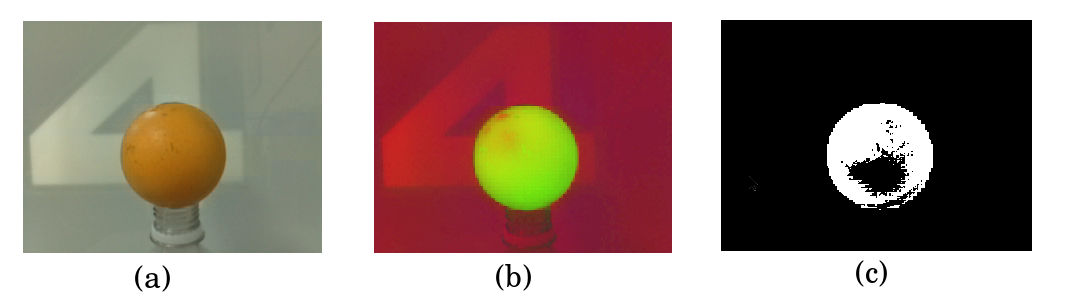
\includegraphics[scale=0.36]{imagenes/HSVyBinaria.jpg}
\caption{(a) imagen original en BGR. (b) imagen original transformada a HSV. (c) imagen binaria a partir de la imagen HSV y el color de la pelota}
\label{fig:proces}
\end{figure}

\begin{figure}[hbtp]
\centering
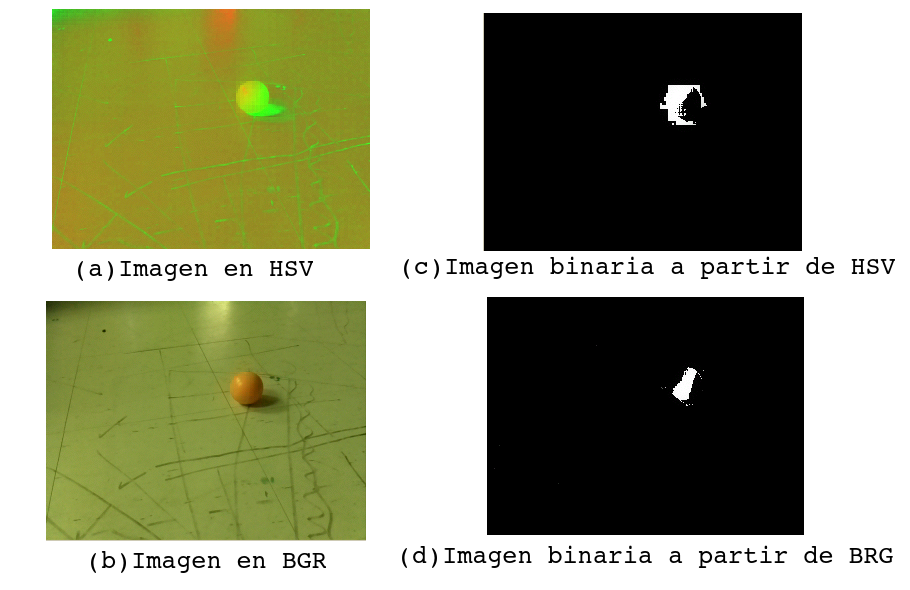
\includegraphics[scale=0.36]{imagenes/compararHSV_BGR.png}
\caption{(a) imagen en HSV. (b) imagen en BGR. (c) imagen binaria a partir de la imagen HSV y el color de la pelota (c) imagen binaria a partir de la imagen en BGR.}
\label{fig:proces}
\end{figure}

Para disminuir el ruido y los posibles elementos aislados que pueda tener la imagen con la que se está trabajando se han aplicado los filtros o transformaciones de morfología en apertura y morfología en clausura de la librería Opencv, basadas en las operaciones básicas de dilatación y erosión. La morfología en apertura es una transformación que consiste en aplicar la operación de erosión seguido de la operación de dilatación. La morfología de clausura es una transformación que aplica la dilatación seguido de la erosión.

De esta forma se logró ubicar la pelota con la cámara Raspberry Pi en el 100\% de las pruebas realizadas, que se describen en el cap\'itulo \ref{chapter:resultados}.


